% !TeX program = pdflatex
% Main document for Overleaf. Edit the report text and tables below.
\documentclass[11pt,a4paper]{article}
\usepackage[T1]{fontenc}
\usepackage[utf8]{inputenc}
\usepackage{lmodern}
\usepackage[a4paper,margin=20mm,includefoot]{geometry}
\usepackage{amsmath,amssymb,textcomp}
\usepackage{booktabs,longtable,array,graphicx,float}
\usepackage[table]{xcolor}
\usepackage{caption}
\usepackage{microtype}
\usepackage{xurl}
\usepackage[hidelinks,unicode]{hyperref}
\usepackage{fancyhdr}
\usepackage{tikz}
\usetikzlibrary{arrows.meta,positioning,calc}
\DeclareUnicodeCharacter{03A3}{\ensuremath{\Sigma}}
\DeclareUnicodeCharacter{0394}{\ensuremath{\Delta}}
\DeclareUnicodeCharacter{2212}{\ensuremath{-}}
\DeclareUnicodeCharacter{00D7}{\ensuremath{\times}}
\DeclareUnicodeCharacter{00B2}{\textsuperscript{2}}
\DeclareUnicodeCharacter{2026}{\ldots{}}
\definecolor{reportblue}{HTML}{244B69}
\setlength{\parindent}{0pt}
\setlength{\parskip}{6pt}
\setlength{\emergencystretch}{3em}
\setlength{\LTpre}{6pt}
\setlength{\LTpost}{6pt}
\captionsetup{font=small,labelfont=bf,skip=6pt}
\pagestyle{fancy}
\fancyhf{}
\renewcommand{\headrulewidth}{0pt}
\renewcommand{\footrulewidth}{0pt}
\fancyfoot[L]{\footnotesize LUSR\quad 32nm\_MGK\quad 0.9 V}
\fancyfoot[R]{\footnotesize\thepage}
\hypersetup{pdftitle={ML Driven PVT Variation Aware Leakage Estimation},
pdfauthor={Dhimant Bhuva, Jal Parikh, Garima Mittal, Krishna Goel}}
\begin{document}
\begin{center}
{\LARGE\bfseries ML Driven PVT Variation Aware\\[4pt]Leakage Estimation\par}
\vspace{10pt}
{\large 8-bit Parity Checker\quad 32nm\_MGK\quad 0.9 V\par}
\vspace{8pt}
Team 8 --- LUSR\\[4pt]
Dhimant Bhuva\enspace\textperiodcentered{}\enspace Jal Parikh\enspace\textperiodcentered{}\enspace Garima Mittal\enspace\textperiodcentered{}\enspace Krishna Goel
\end{center}
Digital VLSI Design --- Course Project. Results generated from the supplied model and the reproducible source package.

\subsection*{Measured outcome}

The project uses 400,000 single-transistor simulations to compare four regression families and selects one four-current model per transistor case. Gate validation covers all 18 input cases at 200 independent PVT corners; full parity validation covers all 256 vectors at those same corners (51,200 complete-netlist operating points).

\begingroup
\fontsize{8.5}{11}\selectfont
\setlength{\tabcolsep}{3pt}
\renewcommand{\arraystretch}{1.16}
\begin{longtable}{@{}>{\raggedright\arraybackslash}p{50.137mm} >{\centering\arraybackslash}p{37.846mm} >{\centering\arraybackslash}p{37.846mm} >{\centering\arraybackslash}p{37.846mm}@{}}
\toprule
\textbf{Evaluation} & \textbf{Median error (\%)} & \textbf{95th-percentile (\%)} & \textbf{Mean accuracy (\%)} \\
\midrule
\endfirsthead
\toprule
\textbf{Evaluation} & \textbf{Median error (\%)} & \textbf{95th-percentile (\%)} & \textbf{Mean accuracy (\%)} \\
\midrule
\endhead
\midrule\multicolumn{4}{r}{\footnotesize Continued on next page}\\
\endfoot
\bottomrule
\endlastfoot
Five-gate aggregate & 0.256 & 1.12 & 99.6350 \\
Complete parity checker & 0.423 & 1.21 & 99.4897 \\
\end{longtable}
\endgroup
\vspace{2pt}

The 99\% mean-accuracy target was met for the complete circuit. Mean accuracy here is \(100(1-\mathrm{MAPE})\), not R².

All 454,800 reference simulations completed and every gate/circuit output passed the digital logic-level checks. Additional fresh-netlist, current-balance and source-power checks are reported below.

The initial 10,000-row-per-case baseline reached 94.2965\% circuit mean accuracy and is discussed here for comparison. This revision follows the brief's explicit permission to increase the sample count. Its 100,000-row-per-case datasets and 200 evaluation corners use a fresh seed, and its test partition was held back until the revised models were frozen. Earlier test results are not presented as independent verification of the revised models.

\clearpage

% === 1. Assignment, design and conventions ===

\section{Assignment, design and conventions}

\begingroup
\fontsize{8.5}{11}\selectfont
\setlength{\tabcolsep}{3pt}
\renewcommand{\arraystretch}{1.16}
\begin{longtable}{@{}>{\raggedright\arraybackslash}p{41.557mm} >{\raggedright\arraybackslash}p{126.334mm}@{}}
\toprule
\textbf{Item} & \textbf{Implemented value} \\
\midrule
\endfirsthead
\toprule
\textbf{Item} & \textbf{Implemented value} \\
\midrule
\endhead
\midrule\multicolumn{2}{r}{\footnotesize Continued on next page}\\
\endfoot
\bottomrule
\endlastfoot
Assigned model & Original \path|models/32nm_MGK.pm| (repository root); SHA256 56710120d5a2ae9e32a1908e1ee29a98f692a1dec0501eed8976ea6e6bea021e \\
Supply and process & VDD 0.9 V nominal, uniform 0.81--0.99 V; five specified process parameters independently \(\pm\)10\% \\
Geometry & Drawn L=32 nm; training W=32--256 nm; fixed gate NMOS W=64 nm, PMOS W=128 nm \\
Temperature & Uniform \(-\)40 to 125 \textdegree{}C; model nominal temperature 27 \textdegree{}C \\
Simulator & ngspice 42; model level=54, version=4.0, handled by ngspice BSIM4v5 implementation \\
Solver options & gmin=1e-18; abstol=1e-18 A; reltol=1e-6; vntol=1e-9 V \\
Parity convention & Eight total received bits. Y=A0 XOR \ldots{} XOR A7; Y=1 means odd parity/error for an expected even-parity word. \\
\end{longtable}
\endgroup
\vspace{2pt}

The team authorized documented choices wherever the brief is silent. A balanced tree of seven XOR operations is implemented using four standard static-CMOS NAND2 cells per XOR: 28 NAND2 cells, 112 transistors. Widths are constant across gates; stacked transistors are not resized. This is a reproducible leakage-study design, with no claim of optimized delay. Diffusion areas/perimeters are left at model/simulator defaults because no layout was supplied.

\begin{figure}[H]
\centering
% Editable TikZ source for the 8-bit parity checker.
% The seven XOR operations each use four NAND2 cells in the implementation.
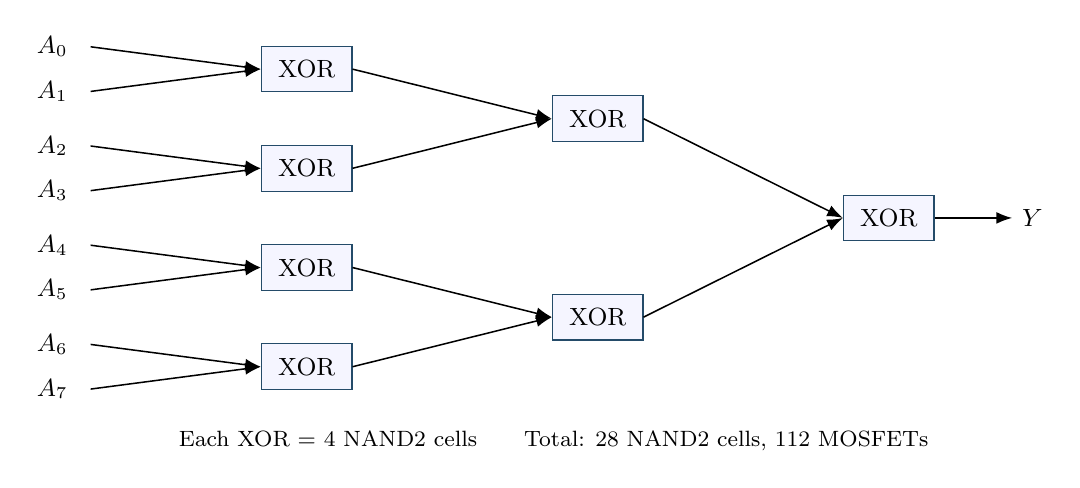
\begin{tikzpicture}[x=1.12cm,y=.63cm,
  xorcell/.style={draw=reportblue,fill=blue!4,minimum width=1.15cm,minimum height=.58cm,font=\small},
  wire/.style={-{Latex[length=2mm]},line width=.55pt},font=\small]
\node[xorcell] (x0) at (3,7) {XOR};
\node[xorcell] (x1) at (3,5) {XOR};
\node[xorcell] (x2) at (3,3) {XOR};
\node[xorcell] (x3) at (3,1) {XOR};
\node[xorcell] (x4) at (6.3,6) {XOR};
\node[xorcell] (x5) at (6.3,2) {XOR};
\node[xorcell] (x6) at (9.6,4) {XOR};
\foreach \i/\target/\yy in {0/x0/7.45,1/x0/6.55,2/x1/5.45,3/x1/4.55,4/x2/3.45,5/x2/2.55,6/x3/1.45,7/x3/.55}{
 \node[anchor=east] at (.4,\yy) {$A_{\i}$};
 \draw[wire] (.55,\yy)--(\target.west);
}
\draw[wire] (x0.east)--(x4.west);
\draw[wire] (x1.east)--(x4.west);
\draw[wire] (x2.east)--(x5.west);
\draw[wire] (x3.east)--(x5.west);
\draw[wire] (x4.east)--(x6.west);
\draw[wire] (x5.east)--(x6.west);
\draw[wire] (x6.east)--(11,4) node[right] {$Y$};
\node[anchor=north,font=\footnotesize,align=center] at (5.8,-.1)
 {Each XOR = 4 NAND2 cells\qquad Total: 28 NAND2 cells, 112 MOSFETs};
\end{tikzpicture}

\caption{A0 is the least-significant bit of vector integers; displayed words read A7\ldots{}A0. Parity detects odd numbers of bit flips, not every multiple-bit error.}
\end{figure}

\clearpage

% === 2. Leakage observable and hierarchy ===

\section{Leakage observable and hierarchy}

The primary observable is total static power supplied by every independent voltage source divided by VDD. With binary rail-valued inputs: \(I_{\mathrm{leak}}=-I(V_{\mathrm{DD}})-\sum_{k\in\mathrm{high}}I(V_{\mathrm{in},k})\). This includes energy supplied through high input drivers when gate tunnelling is present. Supply-only −I(VDD) is also saved as a secondary diagnostic. Summing absolute transistor terminal currents would double-count paths and is not used.

Transistor currents are signed into their terminals and measured using four separate sources. For a source written Vd d 0 VD, \(I_d=-I(V_d)\), with analogous definitions for gate, source and body. KCL requires \(I_d+I_g+I_s+I_b=0\).

For ML energy aggregation, each transistor contributes \(P=(V_d-V_s)I_d+(V_g-V_s)I_g+(V_b-V_s)I_b\). This explicitly closes the source current as \(I_s=-(I_d+I_g+I_b)\). All four raw learned currents and their KCL residual are retained. Source closure avoids a common-mode power artifact from independently predicted currents; it does not enforce KCL at shared circuit nodes or guarantee positive predicted power.

Part B uses recorded SPICE internal/output voltages to form transistor features, exactly as directed by the brief. The voltage columns labelled for ML are copies with provenance, not independent ML voltage predictions. AND2 and OR2 references are complete connected NAND2+INV and NOR2+INV netlists. Part C propagates Boolean inputs through all 28 NAND2 cells, retrieves the matching gate prediction at the same corner, and sums those predictions; complete-circuit internal voltages and measured currents do not enter prediction.

\clearpage

% === 3. Data generation and checks ===

\section{Data generation and checks}

Sampling uses the fixed seed 20261024 and independently generated streams. VDD is drawn before Vd and Vs, which are independent uniform draws conditional on VDD. W, temperature and all five process parameters are sampled independently. PMOS vth0 remains negative; its numeric interval endpoints are sorted. Every evaluation corner contains a shared NMOS process draw and a separate shared PMOS process draw.

\begingroup
\fontsize{8.5}{11}\selectfont
\setlength{\tabcolsep}{3pt}
\renewcommand{\arraystretch}{1.16}
\begin{longtable}{@{}>{\raggedright\arraybackslash}p{27.549mm} >{\centering\arraybackslash}p{21.067mm} >{\centering\arraybackslash}p{21.067mm} >{\raggedright\arraybackslash}p{93.991mm}@{}}
\toprule
\textbf{Case} & \textbf{Gate voltage} & \textbf{Body voltage} & \textbf{Rows / train / validation / test} \\
\midrule
\endfirsthead
\toprule
\textbf{Case} & \textbf{Gate voltage} & \textbf{Body voltage} & \textbf{Rows / train / validation / test} \\
\midrule
\endhead
\midrule\multicolumn{4}{r}{\footnotesize Continued on next page}\\
\endfoot
\bottomrule
\endlastfoot
NMOS ON & VDD & 0 & 100,000 / 70,000 / 15,000 / 15,000 \\
NMOS OFF & 0 & 0 & 100,000 / 70,000 / 15,000 / 15,000 \\
PMOS ON & 0 & VDD & 100,000 / 70,000 / 15,000 / 15,000 \\
PMOS OFF & VDD & VDD & 100,000 / 70,000 / 15,000 / 15,000 \\
\end{longtable}
\endgroup
\vspace{2pt}

A separate supplemental validation set contains 512 independently sampled single-FET PVT/width configurations per case, at exact and near supply rails. These are not added to training, not substituted for the uniform assigned datasets, and not drawn from gate/circuit corners. The seed is 2026102407. Its predefined selection score is MAPE of per-FET dissipated power/VDD on nonzero-bias configurations; the all-terminals-equal physical invariant is reported separately. All raw terminal-current errors remain available. This validation addresses the rail-boundary distribution shift without using any gate or circuit current for model selection.

ON/OFF are the brief's gate-bias labels. Because source voltage varies independently, these labels do not guarantee strong inversion or cutoff at every sampled bias. Each CSV contains vdd,temp,w,vd,vs,vg,vb,vth0,toxe,ndep,u0,xj,id,ig,is,ib, with currents in amperes and SI geometry.

\begingroup
\fontsize{8.5}{11}\selectfont
\setlength{\tabcolsep}{3pt}
\renewcommand{\arraystretch}{1.16}
\begin{longtable}{@{}>{\raggedright\arraybackslash}p{50.137mm} >{\centering\arraybackslash}p{37.846mm} >{\centering\arraybackslash}p{37.846mm} >{\centering\arraybackslash}p{37.846mm}@{}}
\toprule
\textbf{Case} & \textbf{Maximum |\(\Sigma\)I| (A)} & \textbf{Maximum |\(\Sigma\)I|/\(\Sigma\)|I|} & \textbf{Above mixed diagnostic threshold} \\
\midrule
\endfirsthead
\toprule
\textbf{Case} & \textbf{Maximum |\(\Sigma\)I| (A)} & \textbf{Maximum |\(\Sigma\)I|/\(\Sigma\)|I|} & \textbf{Above mixed diagnostic threshold} \\
\midrule
\endhead
\midrule\multicolumn{4}{r}{\footnotesize Continued on next page}\\
\endfoot
\bottomrule
\endlastfoot
nmos\_off & 3.35e-22 & 7.52e-15 & 0 \\
nmos\_on & 1.15e-15 & 9.59e-05 & 225 \\
pmos\_off & 8.11e-15 & 1.42e-04 & 4153 \\
pmos\_on & 3.80e-17 & 3.79e-06 & 1 \\
\end{longtable}
\endgroup
\vspace{2pt}

The diagnostic threshold is 1e-18 A + 1e-6 × \ensuremath{\Sigma}\textbar I\textbar. Some finite-precision SPICE residuals exceed this diagnostic despite successful operating-point convergence. They are reported and retained, not projected out of the reference dataset. The worst normalized residual is 0.01424\%. Spread-out rows were additionally compared with independently instantiated fresh model cards to verify batched parameter updates.

Varying TOXE alone while retaining supplied TOXP and DTOX can trigger the BSIM warning that DTOX is ignored. TOXE remains active, as confirmed by a direct sensitivity experiment. The original model is unchanged; TOXP, TOXM, TOXREF and other unassigned parameters are never silently co-varied.

\clearpage

\subsection*{Controlled physical trends}

Each trend uses 41 points per polarity, with 246 extra fresh SPICE solves total. The illustrative baseline is L=W=32 nm, VDD=0.9 V and T=27 °C, with nominal process values. Only the horizontal-axis parameter changes. This illustrative W does not change the 64/128 nm gate sizing.

\begin{figure}[H]
\centering
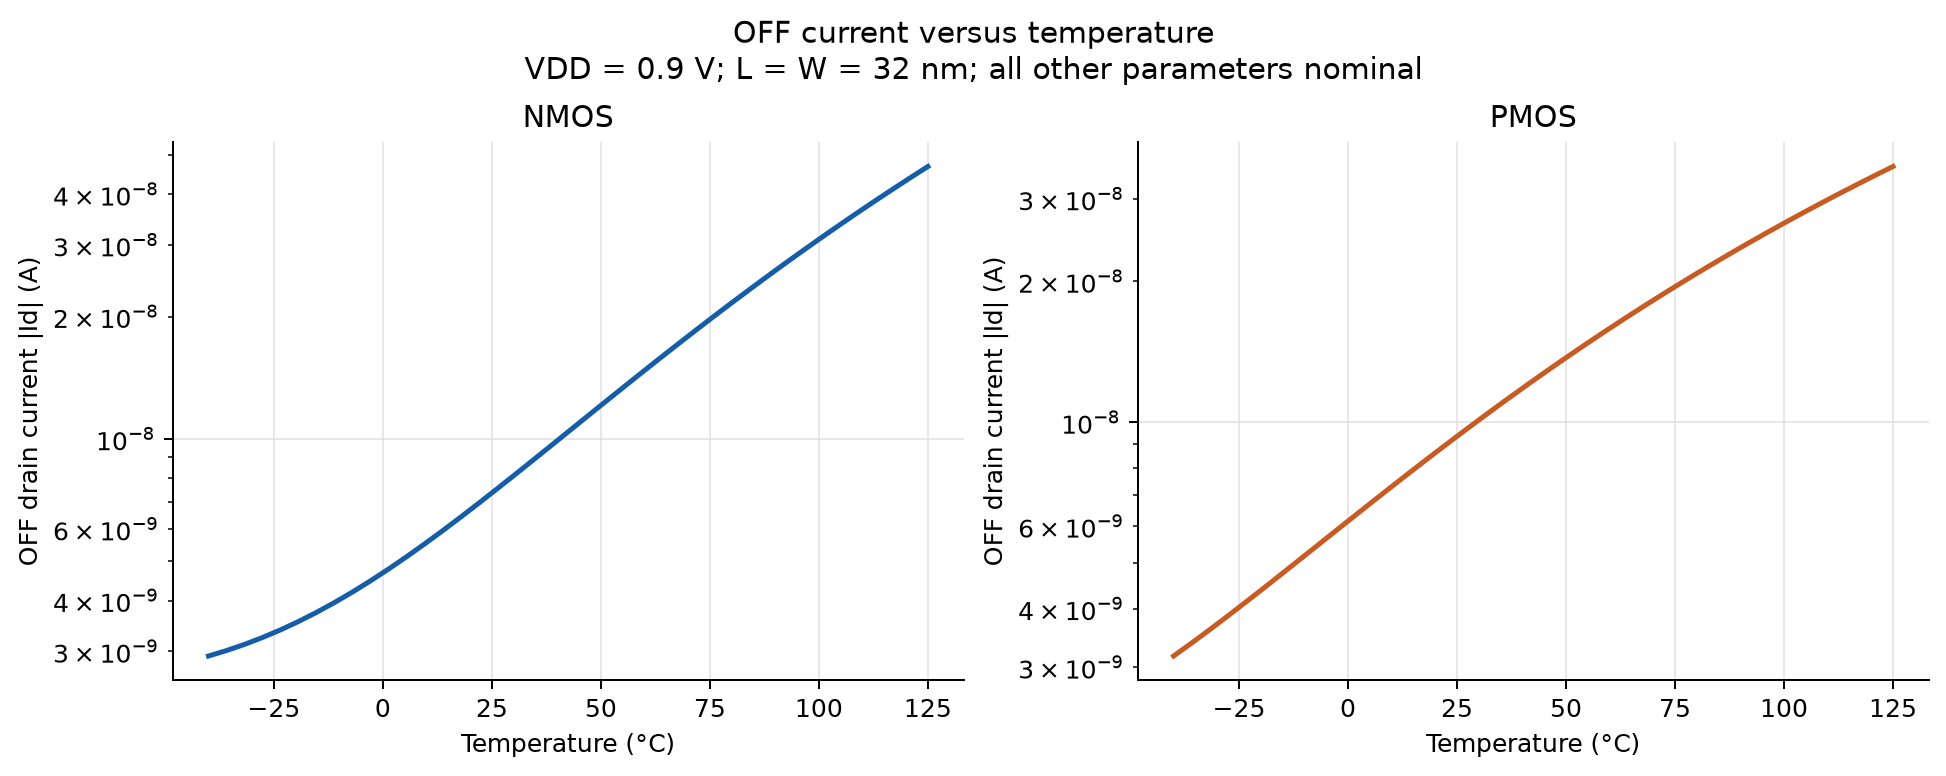
\includegraphics[width=.87\linewidth,height=.20\textheight,keepaspectratio]{data_checks/plots/off_current_vs_temperature.png}
\caption{OFF drain current generally increases with temperature at fixed bias. Other parameters are held constant.}
\end{figure}

\begin{figure}[H]
\centering
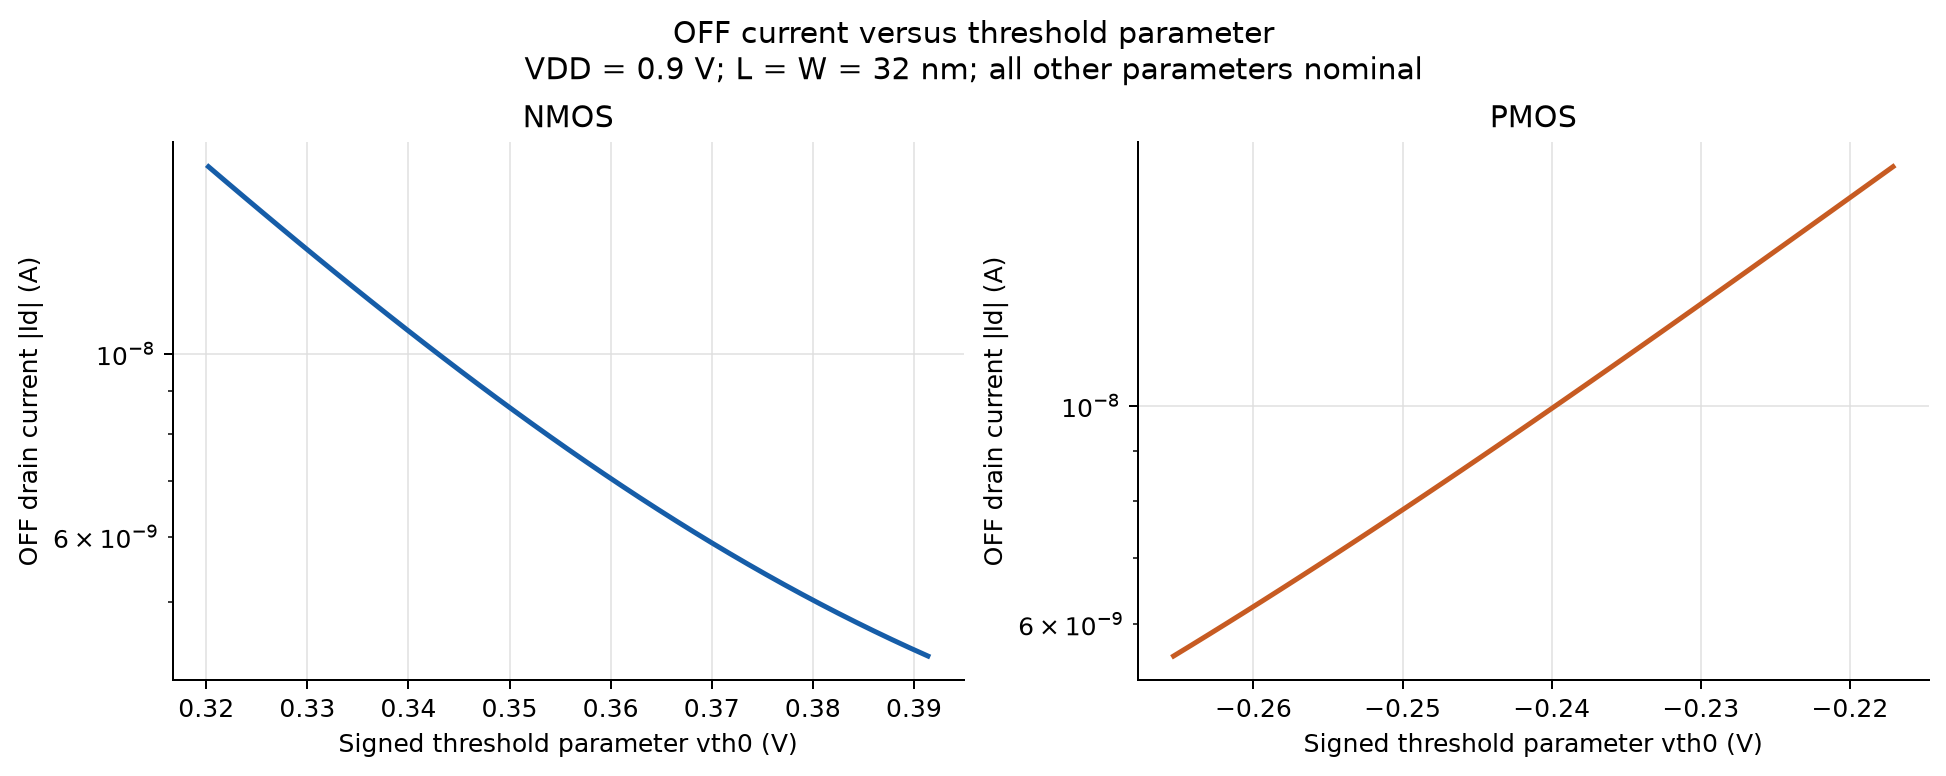
\includegraphics[width=.87\linewidth,height=.20\textheight,keepaspectratio]{data_checks/plots/off_current_vs_vth0.png}
\caption{Increasing threshold magnitude reduces OFF current. PMOS vth0 is plotted with its physical negative sign.}
\end{figure}

\begin{figure}[H]
\centering
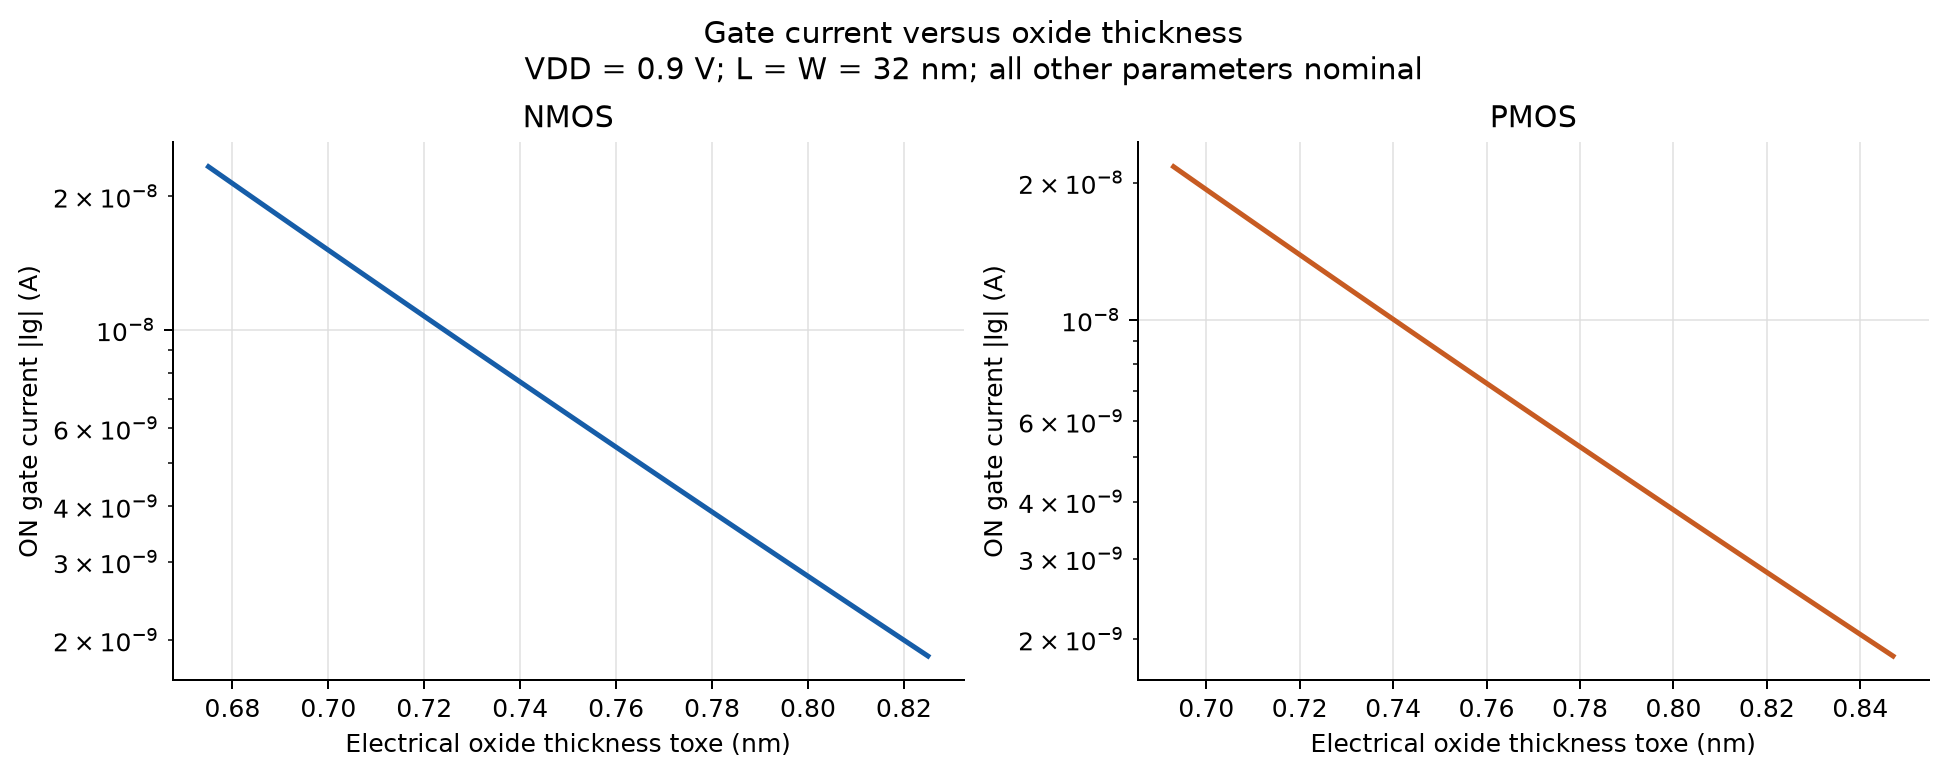
\includegraphics[width=.87\linewidth,height=.20\textheight,keepaspectratio]{data_checks/plots/gate_current_vs_toxe.png}
\caption{ON gate-current magnitude decreases as the electrical oxide thickness increases; supplied remaining oxide parameters are retained.}
\end{figure}

\clearpage

% === 4. Model comparison and held-out evaluation ===

\section{Model comparison and held-out evaluation}

Four families are compared: extra\_trees, hist\_gradient\_boosting, local\_quintic\_rbf, random\_forest. Deterministic voltage, temperature and geometry transformations are computed from the 12 specified inputs. All fitted preprocessing uses training rows only. Validation controls model selection and documented tuning; the test partition is reserved for the selected models. No gate or circuit reference currents are used for fitting or selection.

Selection policy: Minimize the predeclared independent single-FET boundary-validation nonzero-bias power/VDD MAPE; use uniform-validation smooth-component log RMSE only to break ties. The complete uniform-validation raw-current statistics are reported separately. No final-test or gate/circuit leakage is used for selection.

Preprocessing, hyperparameters, validation summaries and the original freeze provenance are recorded in results/ml\_manifest.json and results/revision\_selection.json (paths relative to the repository root). The saved model API accepts the original 12 inputs and returns four raw signed terminal currents. Reloaded predictions are checked against predictions before serialization.

features: Canonical drain/source polarity, voltage coordinates and smooth temperature/\allowbreak{}geometry/\allowbreak{}process functions of the original 12 inputs.

targets: Positive conductance and gate/body magnitudes in logarithms; physical baselines normalize selected targets. Every fitted residual uses 70,000 uniform training rows only.

validation: 15,000 uniform rows plus 512 independent boundary single-FET rows per case; test 15,000 rows remain untouched until all four model files and sources are frozen.

\begingroup
\fontsize{8.5}{11}\selectfont
\setlength{\tabcolsep}{3pt}
\renewcommand{\arraystretch}{1.16}
\begin{longtable}{@{}>{\raggedright\arraybackslash}p{50.521mm} >{\centering\arraybackslash}p{23.682mm} >{\centering\arraybackslash}p{20.524mm} >{\centering\arraybackslash}p{20.524mm} >{\centering\arraybackslash}p{29.997mm} >{\centering\arraybackslash}p{14.209mm}@{}}
\toprule
\textbf{Case / family / variant} & \textbf{Raw R\textsuperscript{2}} & \textbf{Median error (\%)} & \textbf{p95 error (\%)} & \textbf{Boundary power MAPE (\%)} & \textbf{Selected} \\
\midrule
\endfirsthead
\toprule
\textbf{Case / family / variant} & \textbf{Raw R\textsuperscript{2}} & \textbf{Median error (\%)} & \textbf{p95 error (\%)} & \textbf{Boundary power MAPE (\%)} & \textbf{Selected} \\
\midrule
\endhead
\midrule\multicolumn{6}{r}{\footnotesize Continued on next page}\\
\endfoot
\bottomrule
\endlastfoot
nmos\_on / random\_forest / canonical\_log\_targets & 0.954804377 & 11 & 56.5 & 27.1 &  \\
nmos\_on / extra\_trees / canonical\_log\_targets & 0.964358024 & 9.05 & 46.4 & 25.4 &  \\
nmos\_on / hist\_gradient\_boosting / canonical\_log\_targets & 0.995033959 & 2.76 & 19.8 & 4.53 &  \\
nmos\_on / local\_quintic\_rbf / raw; 256 neighbors; ON gate residual & 0.999998977 & 0.0684 & 1.38 & 0.169 & yes \\
nmos\_off / random\_forest / canonical\_log\_targets & 0.9045973 & 2.11 & 42 & 103 &  \\
nmos\_off / extra\_trees / canonical\_log\_targets & 0.890907131 & 1.33 & 33.6 & 83 &  \\
nmos\_off / hist\_gradient\_boosting / canonical\_log\_targets & 0.94866199 & 1.44 & 23.6 & 73.2 &  \\
nmos\_off / local\_quintic\_rbf / junction; 512 neighbors; physics residual & 0.914215306 & 0.00345 & 5.18 & 1.23 & yes \\
pmos\_on / random\_forest / canonical\_log\_targets & 0.96654288 & 9.82 & 50.8 & 25.9 &  \\
pmos\_on / extra\_trees / canonical\_log\_targets & 0.974422506 & 8.34 & 40.7 & 24.7 &  \\
pmos\_on / hist\_gradient\_boosting / canonical\_log\_targets & 0.996941114 & 2.15 & 18.2 & 7.72 &  \\
pmos\_on / local\_quintic\_rbf / raw; 256 neighbors; ON gate residual & 0.999999015 & 0.0361 & 1.08 & 0.316 & yes \\
pmos\_off / random\_forest / canonical\_log\_targets & 0.946907084 & 1.97 & 36.9 & 56 &  \\
pmos\_off / extra\_trees / canonical\_log\_targets & 0.938500803 & 1.32 & 29.7 & 40.3 &  \\
pmos\_off / hist\_gradient\_boosting / canonical\_log\_targets & 0.98163578 & 1.35 & 19.9 & 25.7 &  \\
pmos\_off / local\_quintic\_rbf / junction; 256 neighbors; physics residual & 0.958543185 & 0.0162 & 5.2 & 1.2 & yes \\
\end{longtable}
\endgroup
\vspace{2pt}

The 16-row table compares four families for each case. All rows use the same training and uniform-validation partitions. Raw-current statistics are reported in common units even when the training target representation differs. The selection score, which addresses the project's power/leakage objective, is stated above; a family need not minimize every reported terminal-current statistic.

\begingroup
\fontsize{8.5}{11}\selectfont
\setlength{\tabcolsep}{3pt}
\renewcommand{\arraystretch}{1.16}
\begin{longtable}{@{}>{\raggedright\arraybackslash}p{41.557mm} >{\raggedright\arraybackslash}p{126.334mm}@{}}
\toprule
\textbf{Family} & \textbf{Main hyperparameters} \\
\midrule
\endfirsthead
\toprule
\textbf{Family} & \textbf{Main hyperparameters} \\
\midrule
\endhead
\midrule\multicolumn{2}{r}{\footnotesize Continued on next page}\\
\endfoot
\bottomrule
\endlastfoot
Random forest & 128 trees; all features; unrestricted depth; minimum leaf size 2; seed 20261024. \\
Extra trees & 128 trees; all features; unrestricted depth; minimum leaf size 2; seed 20261024. \\
Histogram gradient boosting & Four target regressors; 400 iterations; rate 0.08; 63 leaves; minimum leaf 15; L2=0.01; seed 20261024. \\
local\_quintic\_rbf & Local quintic RBF, degree 2 polynomial, smoothing 1e-12; 512 neighbors for NMOS OFF; 256 for other cases. ON cases additionally learn a gate-edge log residual using 256 neighbors. \\
\end{longtable}
\endgroup
\vspace{2pt}

Canonical PMOS polarity and ordered drain/source; log positive Gd/Gs and \textbar Ig\textbar/\textbar Ib\textbar, with width normalization; OFF log residuals relative to fixed BSIM gate-edge and diode-shaped body baselines. ON uses a separately learned gate-edge residual with compensating half gate-current changes in Id/Is; learned channel difference and KCL residual preserved. All four currents reconstructed from learned residuals; no SPICE at inference. Exact all-terminal-equal zero invariant.

In ordered, NMOS-polarity coordinates let \(\Delta V=V_{\mathrm{high}}-V_{\mathrm{low}}\) and \(H=\frac{I_g+I_b}{2}\). The learned positive channel quantities are \(G_d=\frac{I_d+H}{\Delta V}\) and \(G_s=-\frac{I_s+H}{\Delta V}\). Training divides these conductances and \textbar Ig\textbar{} by \(\frac{W-10\,\mathrm{nm}}{100\,\mathrm{nm}}\); body current is not width normalized. Natural logarithms handle the dynamic range. The inverse transformation restores signs and the original drain/source ordering. Gd and Gs are separate learned outputs, so raw KCL remains a reported diagnostic.

For OFF cases, the gate-current baseline is the fixed BSIM gate-to-diffusion edge expression using the supplied card parameters; the model learns its logarithmic residual. The body baseline is \(5\times10^{-15}\left[2-\exp\!\left(-\frac{V_{\mathrm{low}}}{V_T}\right)-\exp\!\left(-\frac{V_{\mathrm{high}}}{V_T}\right)\right]\,\mathrm{A}\). This body scale and the junction-coordinate warp are numerical conditioning choices, not exact BSIM body equations. For ON cases, an additional local RBF learns \(\log\!\left(\frac{|I_g|}{|I_{\mathrm{edge,source}}+I_{\mathrm{edge,drain}}|}\right)\); half of its gate-current change is compensated in each drain/source prediction, preserving the learned channel difference and raw KCL residual. At zero edge voltage, tiny gate-body tunnelling is omitted by this ON gate baseline; its raw-current error remains in boundary diagnostics. The fixed coefficients and current reconstruction are implemented in code/lusr/physics\_surrogate.py and code/lusr/smooth\_models.py. The BSIM4 manual is the reference for the gate-edge expressions.

\begingroup
\fontsize{8.5}{11}\selectfont
\setlength{\tabcolsep}{3pt}
\renewcommand{\arraystretch}{1.16}
\begin{longtable}{@{}>{\raggedright\arraybackslash}p{50.137mm} >{\centering\arraybackslash}p{37.846mm} >{\centering\arraybackslash}p{37.846mm} >{\centering\arraybackslash}p{37.846mm}@{}}
\toprule
\textbf{Selected case} & \textbf{Boundary power MAPE (\%)} & \textbf{Boundary median (\%)} & \textbf{Boundary p95 (\%)} \\
\midrule
\endfirsthead
\toprule
\textbf{Selected case} & \textbf{Boundary power MAPE (\%)} & \textbf{Boundary median (\%)} & \textbf{Boundary p95 (\%)} \\
\midrule
\endhead
\midrule\multicolumn{4}{r}{\footnotesize Continued on next page}\\
\endfoot
\bottomrule
\endlastfoot
nmos\_on & 0.169 & 0.114 & 0.444 \\
nmos\_off & 1.23 & 0.216 & 5.52 \\
pmos\_on & 0.316 & 0.19 & 1.05 \\
pmos\_off & 1.2 & 0.196 & 6.2 \\
\end{longtable}
\endgroup
\vspace{2pt}

\begingroup
\fontsize{8.5}{11}\selectfont
\setlength{\tabcolsep}{3pt}
\renewcommand{\arraystretch}{1.16}
\begin{longtable}{@{}>{\raggedright\arraybackslash}p{91.919mm} >{\centering\arraybackslash}p{36.932mm} >{\centering\arraybackslash}p{36.932mm}@{}}
\toprule
\textbf{Selected case / variant} & \textbf{Validation MAPE (\%)} & \textbf{Validation mean accuracy (\%)} \\
\midrule
\endfirsthead
\toprule
\textbf{Selected case / variant} & \textbf{Validation MAPE (\%)} & \textbf{Validation mean accuracy (\%)} \\
\midrule
\endhead
\midrule\multicolumn{3}{r}{\footnotesize Continued on next page}\\
\endfoot
\bottomrule
\endlastfoot
nmos\_on / local\_quintic\_rbf / raw; 256 neighbors; ON gate residual & 0.32 & 99.7 \\
nmos\_off / local\_quintic\_rbf / junction; 512 neighbors; physics residual & 13 & 87 \\
pmos\_on / local\_quintic\_rbf / raw; 256 neighbors; ON gate residual & 0.288 & 99.7 \\
pmos\_off / local\_quintic\_rbf / junction; 256 neighbors; physics residual & 3.13 & 96.9 \\
\end{longtable}
\endgroup
\vspace{2pt}

R² is computed separately for each terminal in raw amperes and uniformly averaged in the summary. It is displayed to nine significant digits; values extremely close to one are rounded. Relative errors pool the four terminal arrays. \(\mathrm{Error}=\frac{|I_{\mathrm{ML}}-I_{\mathrm{SPICE}}|}{\max(|I_{\mathrm{SPICE}}|,10^{-18}\,\mathrm{A})}\); very small signed currents can therefore produce large percentage errors. Per-terminal tables, absolute MAE and RMSE, denominator-floor counts and raw KCL diagnostics are supplied in the CSV results.

\begingroup
\fontsize{8.5}{11}\selectfont
\setlength{\tabcolsep}{3pt}
\renewcommand{\arraystretch}{1.16}
\begin{longtable}{@{}>{\raggedright\arraybackslash}p{72.209mm} >{\centering\arraybackslash}p{25.674mm} >{\centering\arraybackslash}p{32.093mm} >{\centering\arraybackslash}p{33.698mm}@{}}
\toprule
\textbf{Held-out case / selected family} & \textbf{R\textsuperscript{2}} & \textbf{Median error (\%)} & \textbf{95th-percentile (\%)} \\
\midrule
\endfirsthead
\toprule
\textbf{Held-out case / selected family} & \textbf{R\textsuperscript{2}} & \textbf{Median error (\%)} & \textbf{95th-percentile (\%)} \\
\midrule
\endhead
\midrule\multicolumn{4}{r}{\footnotesize Continued on next page}\\
\endfoot
\bottomrule
\endlastfoot
nmos\_on / local\_quintic\_rbf & 0.999999167 & 0.0675 & 1.31 \\
nmos\_off / local\_quintic\_rbf & 0.827376259 & 0.00376 & 4.87 \\
pmos\_on / local\_quintic\_rbf & 0.999998832 & 0.037 & 1.08 \\
pmos\_off / local\_quintic\_rbf & 0.969319316 & 0.0137 & 4.77 \\
\end{longtable}
\endgroup
\vspace{2pt}

\begingroup
\fontsize{8.5}{11}\selectfont
\setlength{\tabcolsep}{3pt}
\renewcommand{\arraystretch}{1.16}
\begin{longtable}{@{}>{\raggedright\arraybackslash}p{91.919mm} >{\centering\arraybackslash}p{36.932mm} >{\centering\arraybackslash}p{36.932mm}@{}}
\toprule
\textbf{Held-out case} & \textbf{Pooled terminal-current MAPE (\%)} & \textbf{Single-FET power/VDD MAPE (\%)} \\
\midrule
\endfirsthead
\toprule
\textbf{Held-out case} & \textbf{Pooled terminal-current MAPE (\%)} & \textbf{Single-FET power/VDD MAPE (\%)} \\
\midrule
\endhead
\midrule\multicolumn{3}{r}{\footnotesize Continued on next page}\\
\endfoot
\bottomrule
\endlastfoot
nmos\_on & 0.307 & 0.241 \\
nmos\_off & 4.02 & 0.0947 \\
pmos\_on & 0.278 & 0.169 \\
pmos\_off & 16.6 & 0.126 \\
\end{longtable}
\endgroup
\vspace{2pt}

The project's 99\% target is assessed against circuit leakage, with the same defined source-power observable used throughout. It is not a claim that every signed terminal current has less than 1\% relative error. OFF-current cancellation and tiny body currents can yield large raw-current percentage errors even when their effect on dissipated power is small. Body currents have physical temperature/bias dependence as well as numerical sensitivity near cancellation. Both metrics are reported above; no terminal, corner or input vector is excluded to improve the circuit result.

\clearpage

\subsection*{NMOS ON --- test predictions}

\begin{figure}[H]
\centering
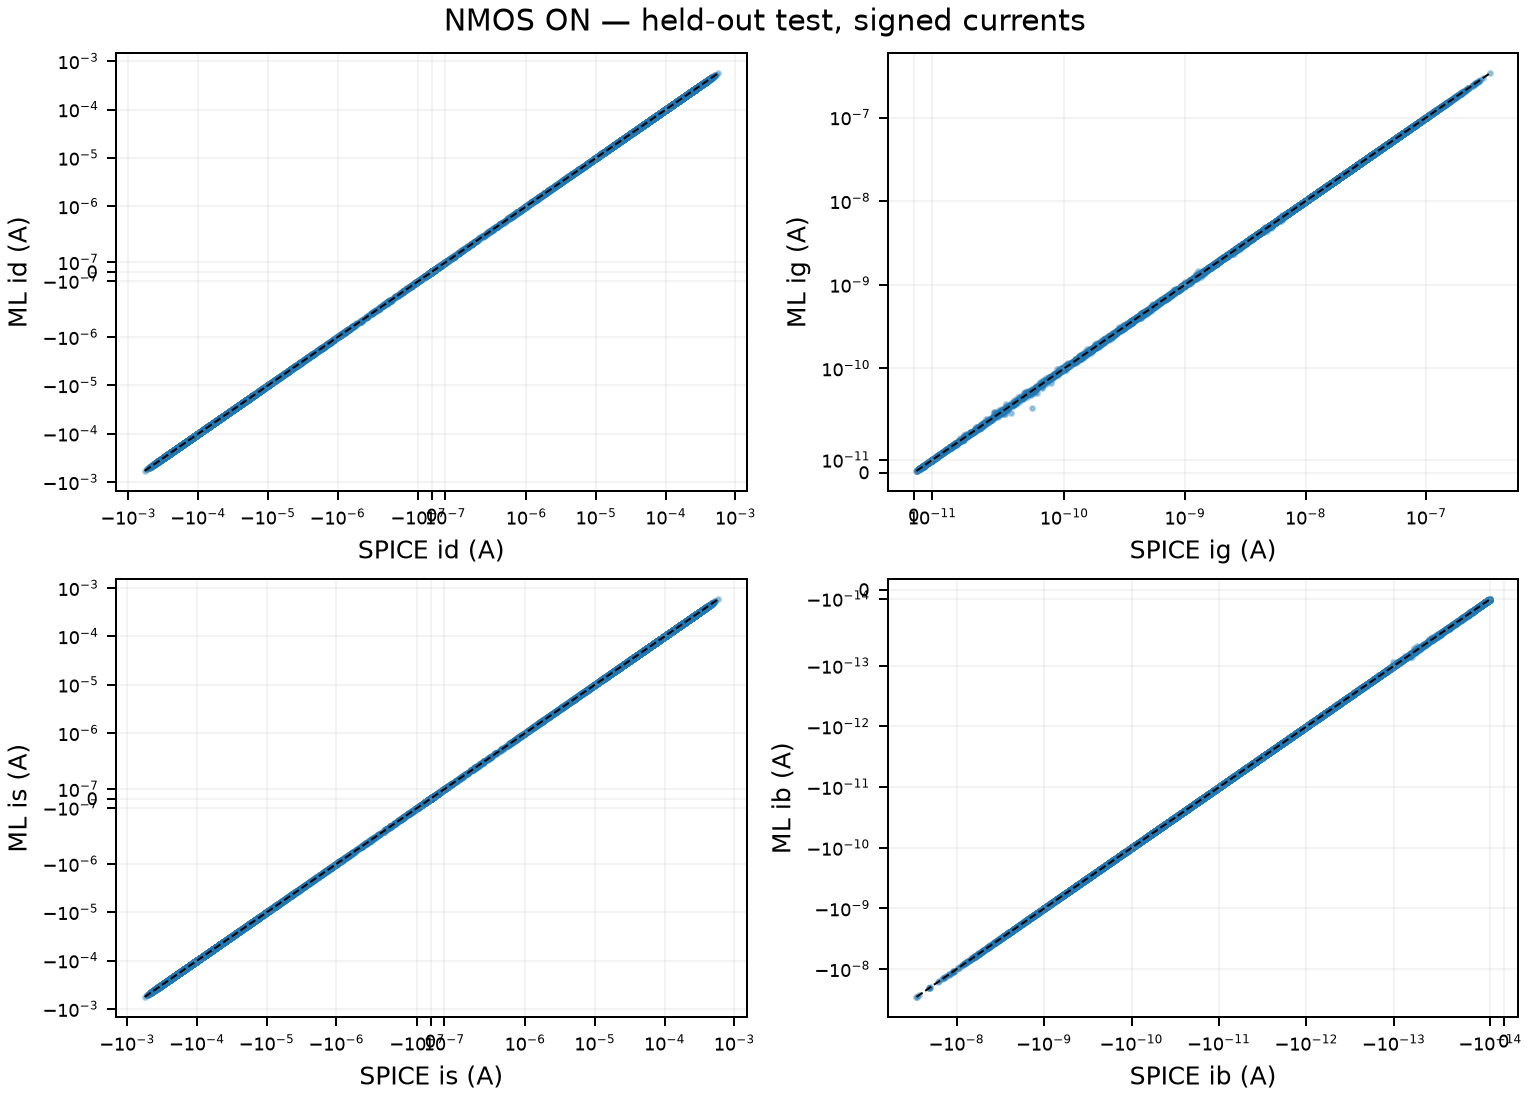
\includegraphics[width=.95\linewidth,height=.49\textheight,keepaspectratio]{figures/nmos_on_parity.png}
\caption{Each panel includes all 15,000 held-out rows. Symmetric-log axes retain negative current predictions and measured signs. Dashed line denotes equality. No point is removed for poor accuracy.}
\end{figure}

\begingroup
\fontsize{8.5}{11}\selectfont
\setlength{\tabcolsep}{3pt}
\renewcommand{\arraystretch}{1.16}
\begin{longtable}{@{}>{\raggedright\arraybackslash}p{30.095mm} >{\centering\arraybackslash}p{26.927mm} >{\centering\arraybackslash}p{33.263mm} >{\centering\arraybackslash}p{34.847mm} >{\centering\arraybackslash}p{36.431mm}@{}}
\toprule
\textbf{Terminal} & \textbf{R\textsuperscript{2}} & \textbf{MAE (A)} & \textbf{Median error (\%)} & \textbf{95th-percentile (\%)} \\
\midrule
\endfirsthead
\toprule
\textbf{Terminal} & \textbf{R\textsuperscript{2}} & \textbf{MAE (A)} & \textbf{Median error (\%)} & \textbf{95th-percentile (\%)} \\
\midrule
\endhead
\midrule\multicolumn{5}{r}{\footnotesize Continued on next page}\\
\endfoot
\bottomrule
\endlastfoot
id & 0.999999308 & 6.04e-08 & 0.0703 & 1.09 \\
ig & 0.999999002 & 1.18e-11 & 0.0593 & 2.22 \\
is & 0.999999308 & 6.04e-08 & 0.0703 & 1.09 \\
ib & 0.99999905 & 8.22e-14 & 0.072 & 0.963 \\
\end{longtable}
\endgroup
\vspace{2pt}

\clearpage

\subsection*{NMOS OFF --- test predictions}

\begin{figure}[H]
\centering
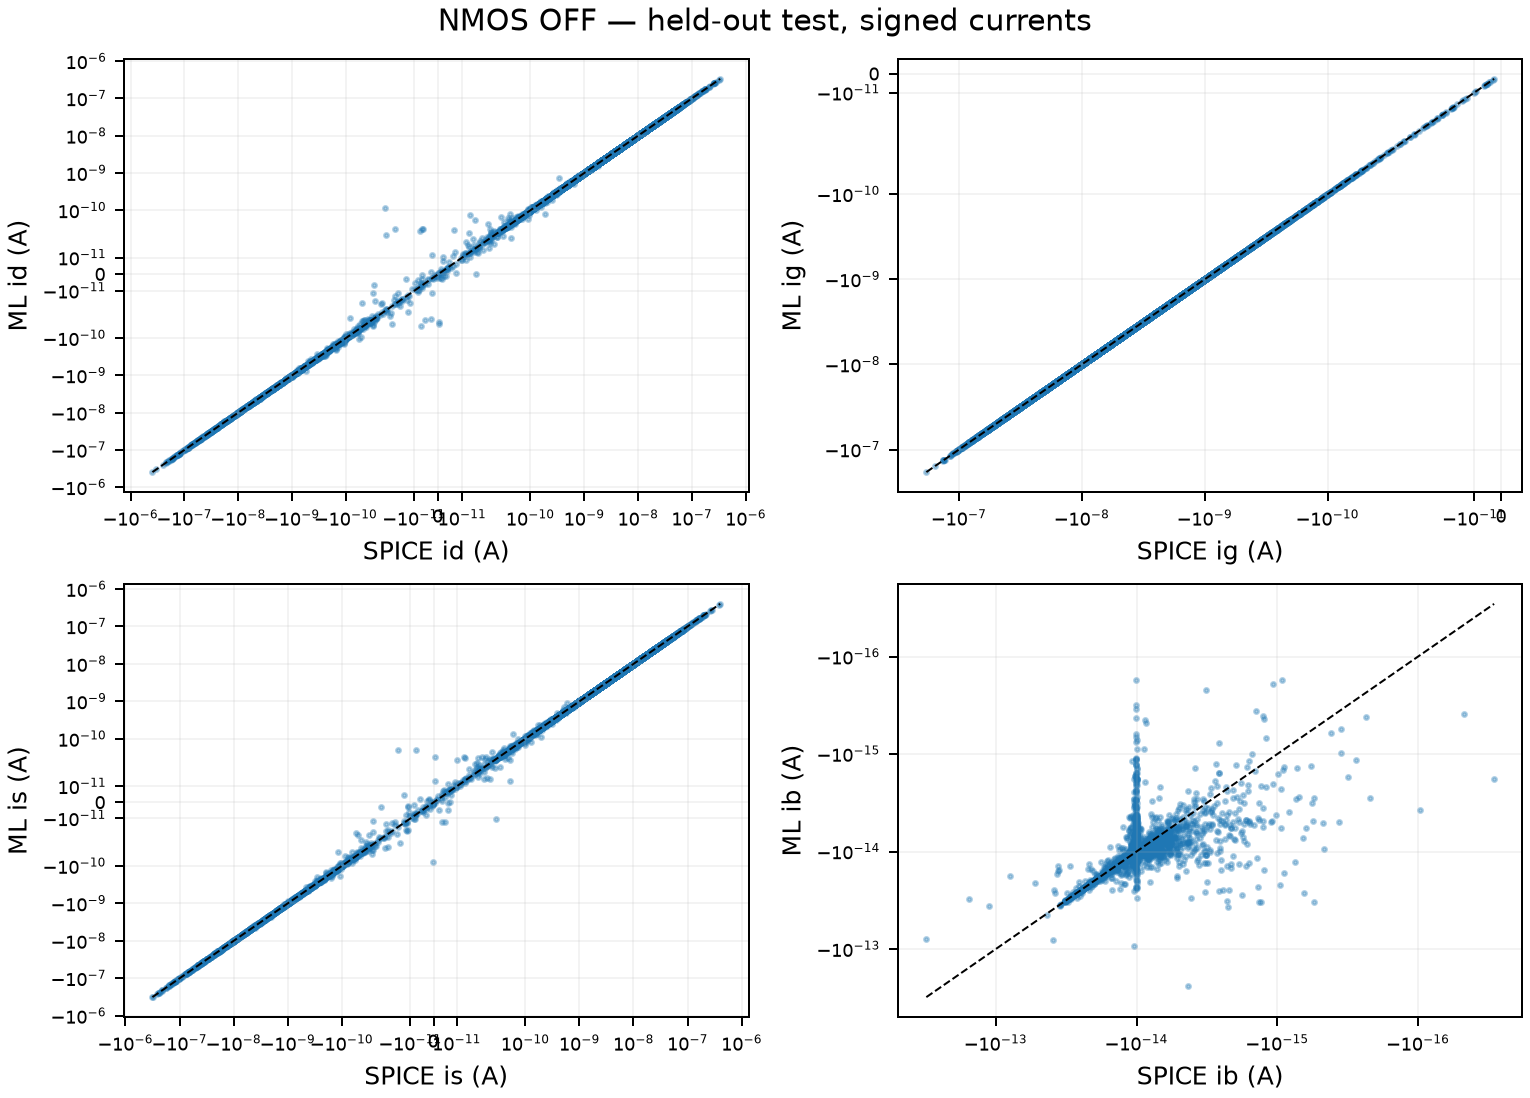
\includegraphics[width=.95\linewidth,height=.49\textheight,keepaspectratio]{figures/nmos_off_parity.png}
\caption{Each panel includes all 15,000 held-out rows. Symmetric-log axes retain negative current predictions and measured signs. Dashed line denotes equality. No point is removed for poor accuracy.}
\end{figure}

\begingroup
\fontsize{8.5}{11}\selectfont
\setlength{\tabcolsep}{3pt}
\renewcommand{\arraystretch}{1.16}
\begin{longtable}{@{}>{\raggedright\arraybackslash}p{30.095mm} >{\centering\arraybackslash}p{26.927mm} >{\centering\arraybackslash}p{33.263mm} >{\centering\arraybackslash}p{34.847mm} >{\centering\arraybackslash}p{36.431mm}@{}}
\toprule
\textbf{Terminal} & \textbf{R\textsuperscript{2}} & \textbf{MAE (A)} & \textbf{Median error (\%)} & \textbf{95th-percentile (\%)} \\
\midrule
\endfirsthead
\toprule
\textbf{Terminal} & \textbf{R\textsuperscript{2}} & \textbf{MAE (A)} & \textbf{Median error (\%)} & \textbf{95th-percentile (\%)} \\
\midrule
\endhead
\midrule\multicolumn{5}{r}{\footnotesize Continued on next page}\\
\endfoot
\bottomrule
\endlastfoot
id & 0.999981236 & 1.40e-11 & 0.0216 & 2.58 \\
ig & 1 & 1.27e-17 & 2.77e-08 & 5.02e-07 \\
is & 0.999981525 & 1.40e-11 & 0.0205 & 2.72 \\
ib & 0.309542275 & 4.54e-16 & 0.0843 & 26.4 \\
\end{longtable}
\endgroup
\vspace{2pt}

\clearpage

\subsection*{PMOS ON --- test predictions}

\begin{figure}[H]
\centering
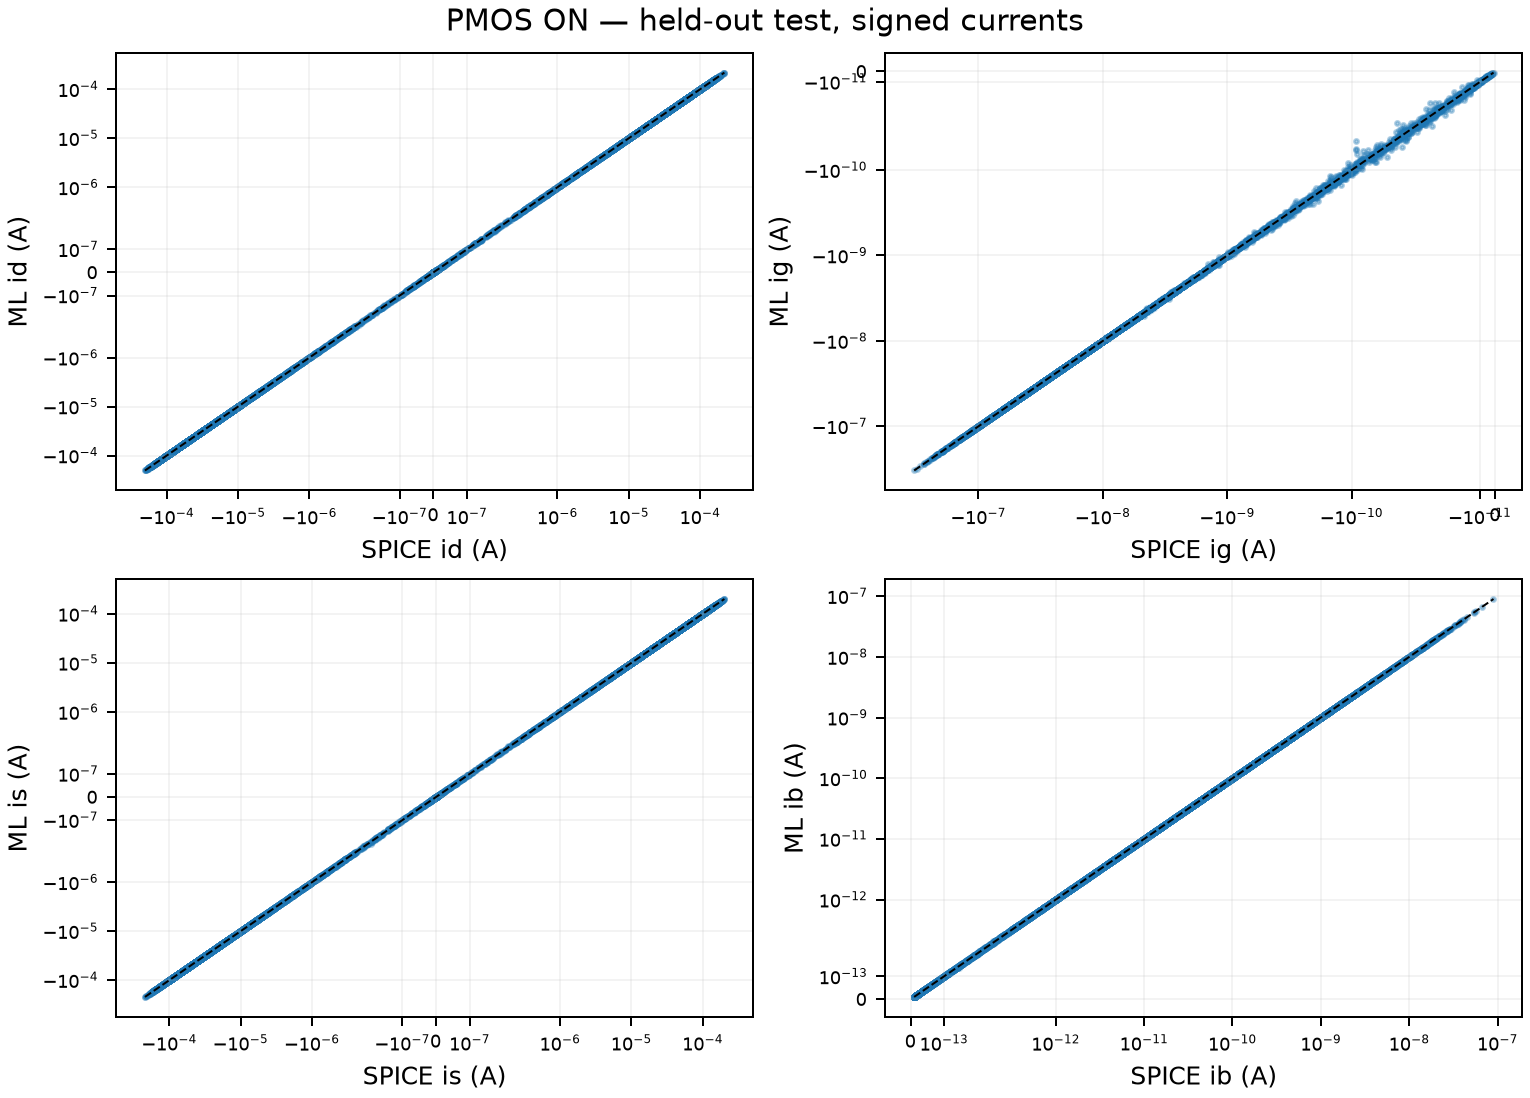
\includegraphics[width=.95\linewidth,height=.49\textheight,keepaspectratio]{figures/pmos_on_parity.png}
\caption{Each panel includes all 15,000 held-out rows. Symmetric-log axes retain negative current predictions and measured signs. Dashed line denotes equality. No point is removed for poor accuracy.}
\end{figure}

\begingroup
\fontsize{8.5}{11}\selectfont
\setlength{\tabcolsep}{3pt}
\renewcommand{\arraystretch}{1.16}
\begin{longtable}{@{}>{\raggedright\arraybackslash}p{30.095mm} >{\centering\arraybackslash}p{26.927mm} >{\centering\arraybackslash}p{33.263mm} >{\centering\arraybackslash}p{34.847mm} >{\centering\arraybackslash}p{36.431mm}@{}}
\toprule
\textbf{Terminal} & \textbf{R\textsuperscript{2}} & \textbf{MAE (A)} & \textbf{Median error (\%)} & \textbf{95th-percentile (\%)} \\
\midrule
\endfirsthead
\toprule
\textbf{Terminal} & \textbf{R\textsuperscript{2}} & \textbf{MAE (A)} & \textbf{Median error (\%)} & \textbf{95th-percentile (\%)} \\
\midrule
\endhead
\midrule\multicolumn{5}{r}{\footnotesize Continued on next page}\\
\endfoot
\bottomrule
\endlastfoot
id & 0.999999726 & 1.39e-08 & 0.0303 & 0.816 \\
ig & 0.999998348 & 1.43e-11 & 0.0571 & 3.39 \\
is & 0.999999726 & 1.39e-08 & 0.0302 & 0.815 \\
ib & 0.999997528 & 4.20e-13 & 0.0337 & 0.704 \\
\end{longtable}
\endgroup
\vspace{2pt}

\clearpage

\subsection*{PMOS OFF --- test predictions}

\begin{figure}[H]
\centering
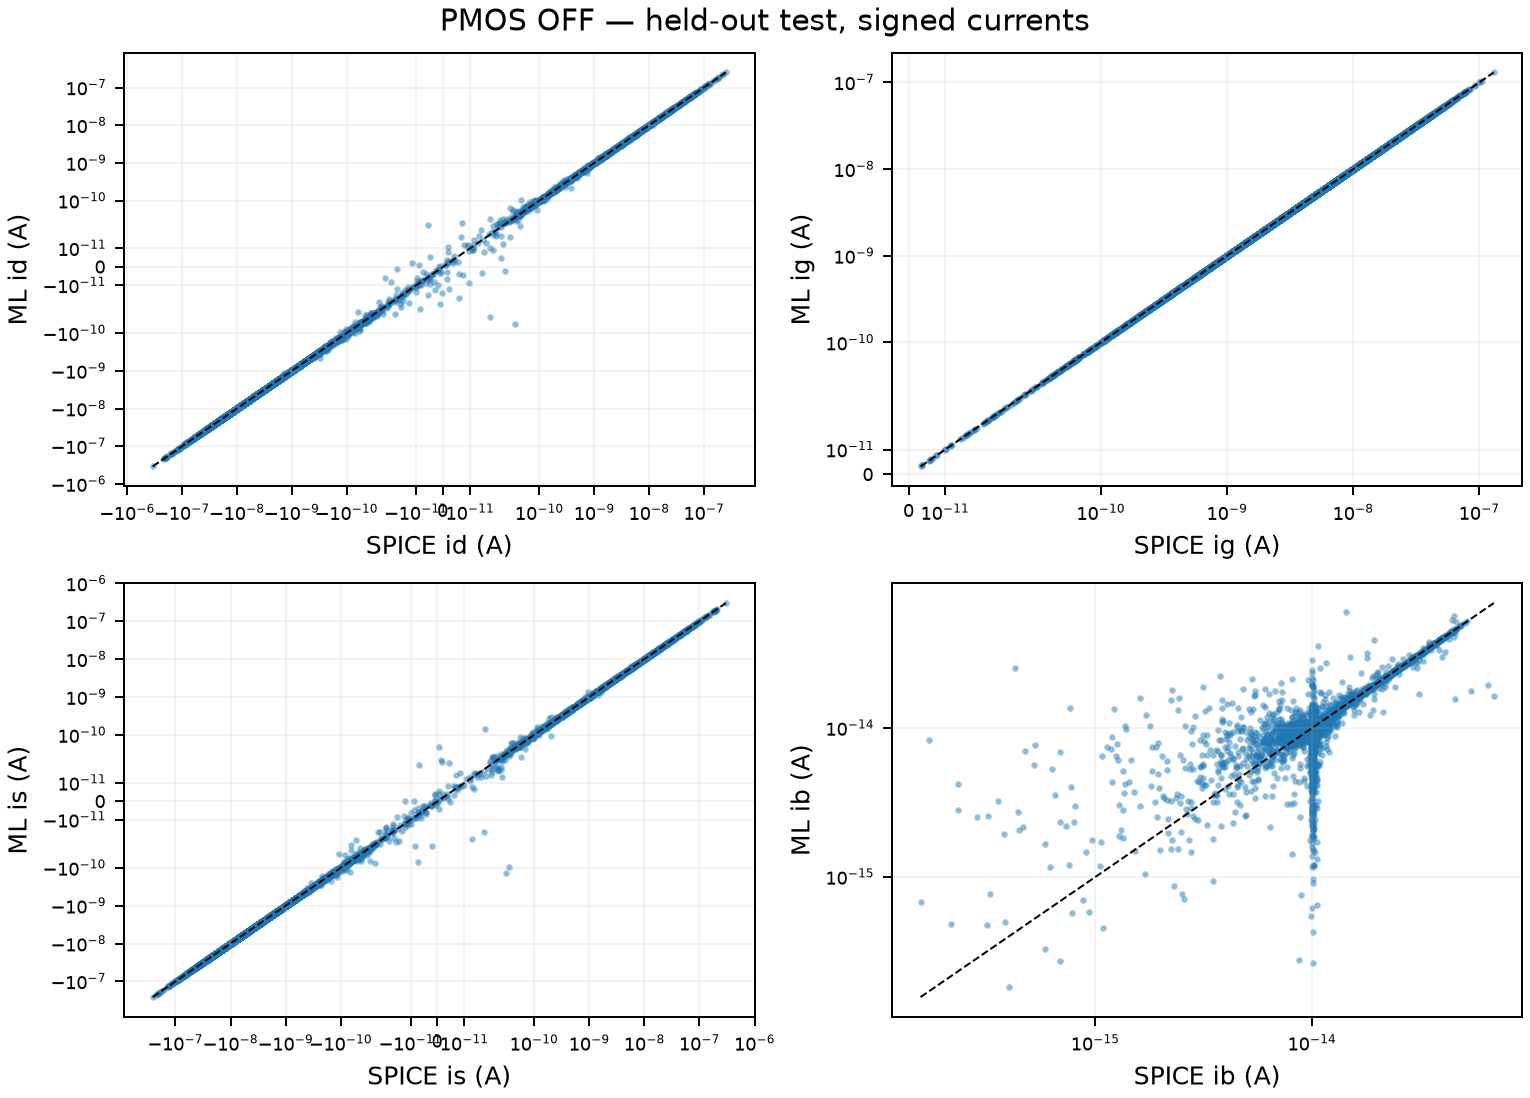
\includegraphics[width=.95\linewidth,height=.49\textheight,keepaspectratio]{figures/pmos_off_parity.png}
\caption{Each panel includes all 15,000 held-out rows. Symmetric-log axes retain negative current predictions and measured signs. Dashed line denotes equality. No point is removed for poor accuracy.}
\end{figure}

\begingroup
\fontsize{8.5}{11}\selectfont
\setlength{\tabcolsep}{3pt}
\renewcommand{\arraystretch}{1.16}
\begin{longtable}{@{}>{\raggedright\arraybackslash}p{30.095mm} >{\centering\arraybackslash}p{26.927mm} >{\centering\arraybackslash}p{33.263mm} >{\centering\arraybackslash}p{34.847mm} >{\centering\arraybackslash}p{36.431mm}@{}}
\toprule
\textbf{Terminal} & \textbf{R\textsuperscript{2}} & \textbf{MAE (A)} & \textbf{Median error (\%)} & \textbf{95th-percentile (\%)} \\
\midrule
\endfirsthead
\toprule
\textbf{Terminal} & \textbf{R\textsuperscript{2}} & \textbf{MAE (A)} & \textbf{Median error (\%)} & \textbf{95th-percentile (\%)} \\
\midrule
\endhead
\midrule\multicolumn{5}{r}{\footnotesize Continued on next page}\\
\endfoot
\bottomrule
\endlastfoot
id & 0.999977133 & 1.36e-11 & 0.0202 & 2.83 \\
ig & 1 & 8.45e-16 & 1.27e-05 & 4.54e-04 \\
is & 0.999976985 & 1.36e-11 & 0.0207 & 2.92 \\
ib & 0.877323146 & 3.96e-16 & 0.154 & 25.7 \\
\end{longtable}
\endgroup
\vspace{2pt}

\clearpage

% === 5. Gate-level validation ===

\section{Gate-level validation}

Each row below summarizes 200 independent corners. SPICE/ML medians are expressed in nA; bias is mean signed ML−SPICE in nA. The same source-power definition is used on both sides. These 3,600 cases are evaluation-only.

\begingroup
\fontsize{8.5}{11}\selectfont
\setlength{\tabcolsep}{3pt}
\renewcommand{\arraystretch}{1.16}
\begin{longtable}{@{}>{\raggedright\arraybackslash}p{25.557mm} >{\centering\arraybackslash}p{22.478mm} >{\centering\arraybackslash}p{22.478mm} >{\centering\arraybackslash}p{18.783mm} >{\centering\arraybackslash}p{22.478mm} >{\centering\arraybackslash}p{21.247mm} >{\centering\arraybackslash}p{24.326mm}@{}}
\toprule
\textbf{Gate / input} & \textbf{SPICE median (nA)} & \textbf{ML median (nA)} & \textbf{Bias (nA)} & \textbf{Median error (\%)} & \textbf{p95 error (\%)} & \textbf{Mean accuracy (\%)} \\
\midrule
\endfirsthead
\toprule
\textbf{Gate / input} & \textbf{SPICE median (nA)} & \textbf{ML median (nA)} & \textbf{Bias (nA)} & \textbf{Median error (\%)} & \textbf{p95 error (\%)} & \textbf{Mean accuracy (\%)} \\
\midrule
\endhead
\midrule\multicolumn{7}{r}{\footnotesize Continued on next page}\\
\endfoot
\bottomrule
\endlastfoot
AND2 00 & 197 & 197 & -4.72e-04 & 0.177 & 0.621 & 99.7667 \\
AND2 01 & 218 & 217 & -0.789 & 0.334 & 0.939 & 99.6038 \\
AND2 10 & 171 & 171 & -0.635 & 0.325 & 0.917 & 99.6216 \\
AND2 11 & 283 & 282 & -1.23 & 0.439 & 1.31 & 99.4843 \\
INV 0 & 81.2 & 81.5 & 0.00375 & 0.313 & 1.14 & 99.6047 \\
INV 1 & 96.8 & 96.8 & 0.24 & 0.315 & 1.53 & 99.5419 \\
NAND2 00 & 86 & 86.1 & 0.234 & 0.206 & 0.55 & 99.7797 \\
NAND2 01 & 110 & 111 & 0.0795 & 0.257 & 0.793 & 99.6983 \\
NAND2 10 & 64.7 & 64.9 & 0.0524 & 0.18 & 0.646 & 99.7745 \\
NAND2 11 & 193 & 193 & 0.466 & 0.32 & 1.57 & 99.5516 \\
NOR2 00 & 162 & 163 & 3.77e-04 & 0.307 & 1.18 & 99.6098 \\
NOR2 01 & 145 & 145 & 0.389 & 0.199 & 1.02 & 99.6917 \\
NOR2 10 & 76.3 & 76.4 & 0.0511 & 0.172 & 0.77 & 99.7311 \\
NOR2 11 & 62.9 & 62.7 & 0.135 & 0.197 & 0.702 & 99.7249 \\
OR2 00 & 271 & 268 & -3.57 & 0.709 & 2.12 & 99.1430 \\
OR2 01 & 226 & 226 & -0.109 & 0.245 & 0.762 & 99.6971 \\
OR2 10 & 165 & 165 & -0.37 & 0.26 & 0.88 & 99.6678 \\
OR2 11 & 158 & 158 & -0.0173 & 0.215 & 0.736 & 99.7379 \\
\end{longtable}
\endgroup
\vspace{2pt}

By median relative error, the most accurate case is NOR2 10 (0.172\%); the least accurate is OR2 00 (0.709\%). The aggregate mean accuracy is 99.6\%.

All 18 gate/input cases individually exceed 99\% mean accuracy over their 200 corners. The lowest is OR2 00, at 99.142956\%.

\clearpage

\subsection*{Gate leakage parity plot}

\begin{figure}[H]
\centering
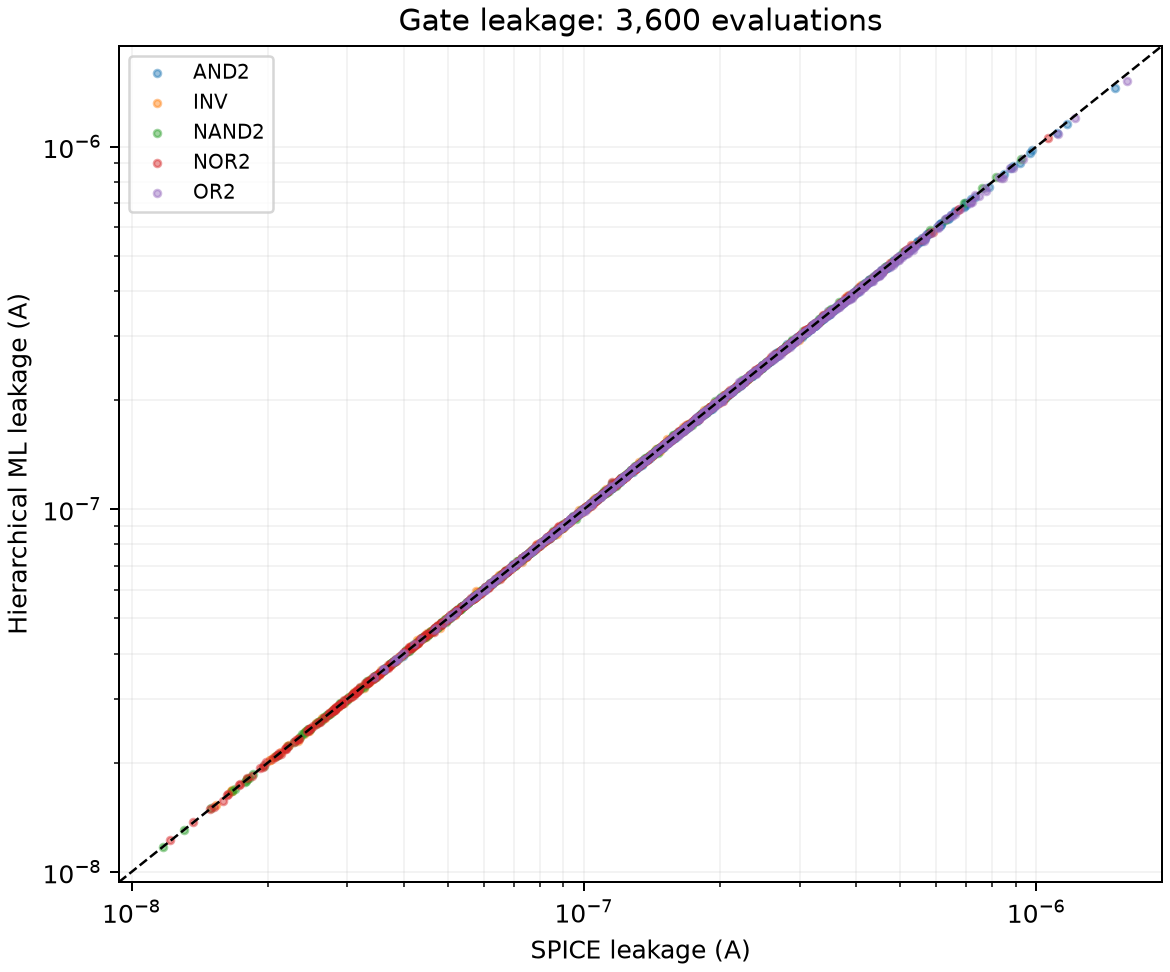
\includegraphics[width=.90\linewidth,height=.62\textheight,keepaspectratio]{figures/gate_parity.png}
\caption{All positive gate predictions on logarithmic axes. Any nonpositive predictions are counted explicitly and remain in all numerical metrics.}
\end{figure}

\clearpage

% === 6. Complete parity checker ===

\section{Complete parity checker}

The SPICE reference is one connected 112-transistor netlist, with all 256 patterns at each of the same 200 corners. Every output was checked against the independently propagated Boolean parity and the 0.2VDD/0.8VDD low/high limits. The complete 256-row per-vector metric table is results/circuit\_metrics\_by\_vector.csv.

\begingroup
\fontsize{8.5}{11}\selectfont
\setlength{\tabcolsep}{3pt}
\renewcommand{\arraystretch}{1.16}
\begin{longtable}{@{}>{\raggedright\arraybackslash}p{58.607mm} >{\centering\arraybackslash}p{25.344mm} >{\centering\arraybackslash}p{25.344mm} >{\centering\arraybackslash}p{26.927mm} >{\centering\arraybackslash}p{25.344mm}@{}}
\toprule
\textbf{Comparison} & \textbf{Median error (\%)} & \textbf{p95 error (\%)} & \textbf{Mean accuracy (\%)} & \textbf{R\textsuperscript{2}} \\
\midrule
\endfirsthead
\toprule
\textbf{Comparison} & \textbf{Median error (\%)} & \textbf{p95 error (\%)} & \textbf{Mean accuracy (\%)} & \textbf{R\textsuperscript{2}} \\
\midrule
\endhead
\midrule\multicolumn{5}{r}{\footnotesize Continued on next page}\\
\endfoot
\bottomrule
\endlastfoot
Hierarchical ML vs full SPICE & 0.423 & 1.21 & 99.4897 & 0.99959365 \\
Standalone SPICE gate sum vs full SPICE & 0.226 & 1.13 & 99.6351 & 0.999636596 \\
Hierarchical ML vs standalone SPICE sum & 0.222 & 0.719 & 99.7334 & 0.999952272 \\
\end{longtable}
\endgroup
\vspace{2pt}

The second row is an evaluation-only diagnostic: it sums true standalone gate leakages using the same Boolean states. It quantifies error introduced by ideal-rail inputs and ignored inter-gate loading even if the transistor surrogate were perfect. It is never substituted for an ML prediction. The third row isolates the surrogate's discrepancy from the standalone-gate reference sum.

Complete-circuit SPICE median=3.62e+03 nA; ML median=3.6e+03 nA; signed mean bias=-13.5 nA. Nonpositive circuit predictions: 0.

\begin{figure}[H]
\centering
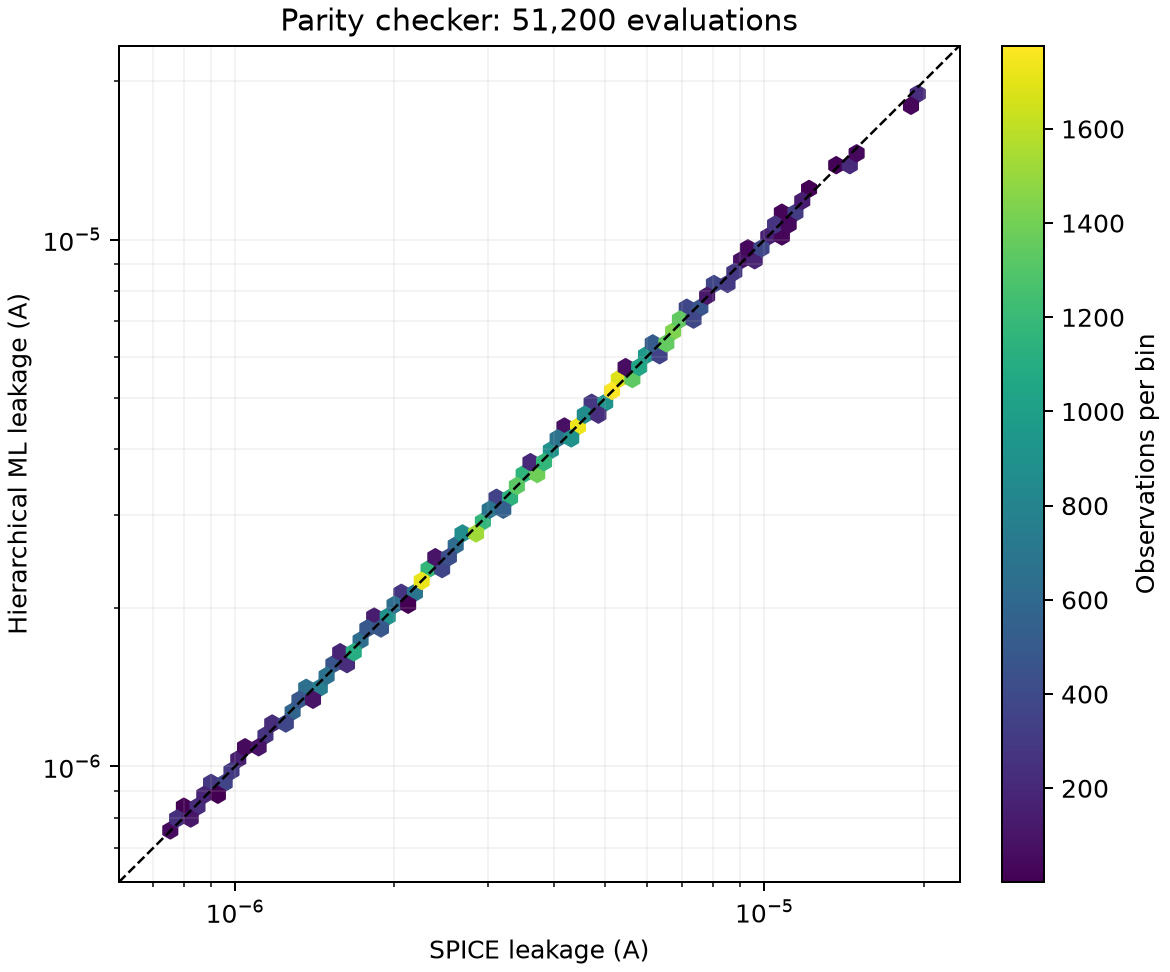
\includegraphics[width=.74\linewidth,height=.42\textheight,keepaspectratio]{figures/circuit_parity.png}
\caption{Complete-circuit comparison over 51,200 observations. Logarithmic binning shows sample density; all observations remain in the result CSV.}
\end{figure}

\clearpage

% === 7. Error analysis and numerical validation ===

\section{Error analysis and numerical validation}

\begingroup
\fontsize{8.5}{11}\selectfont
\setlength{\tabcolsep}{3pt}
\renewcommand{\arraystretch}{1.16}
\begin{longtable}{@{}>{\raggedright\arraybackslash}p{30.095mm} >{\centering\arraybackslash}p{26.927mm} >{\centering\arraybackslash}p{33.263mm} >{\centering\arraybackslash}p{34.847mm} >{\centering\arraybackslash}p{36.431mm}@{}}
\toprule
\textbf{Gate / input} & \textbf{Corner} & \textbf{Temperature (\textdegree{}C)} & \textbf{VDD (V)} & \textbf{Absolute relative error (\%)} \\
\midrule
\endfirsthead
\toprule
\textbf{Gate / input} & \textbf{Corner} & \textbf{Temperature (\textdegree{}C)} & \textbf{VDD (V)} & \textbf{Absolute relative error (\%)} \\
\midrule
\endhead
\midrule\multicolumn{5}{r}{\footnotesize Continued on next page}\\
\endfoot
\bottomrule
\endlastfoot
OR2 00 & 94 & 125 & 0.963 & 4.23 \\
OR2 00 & 77 & 109 & 0.982 & 3.33 \\
INV 0 & 16 & 12.8 & 0.976 & 3.12 \\
NOR2 00 & 16 & 12.8 & 0.976 & 3.11 \\
OR2 00 & 46 & 107 & 0.943 & 3.09 \\
\end{longtable}
\endgroup
\vspace{2pt}

The largest-error rows and their corner identifiers are retained in results/worst\_gate\_cases.csv and worst\_circuit\_cases.csv. Full corner records provide both polarities' process values. The scatter below shows association with PVT parameters, not a controlled causal experiment: other sampled parameters vary simultaneously.

\begin{figure}[H]
\centering
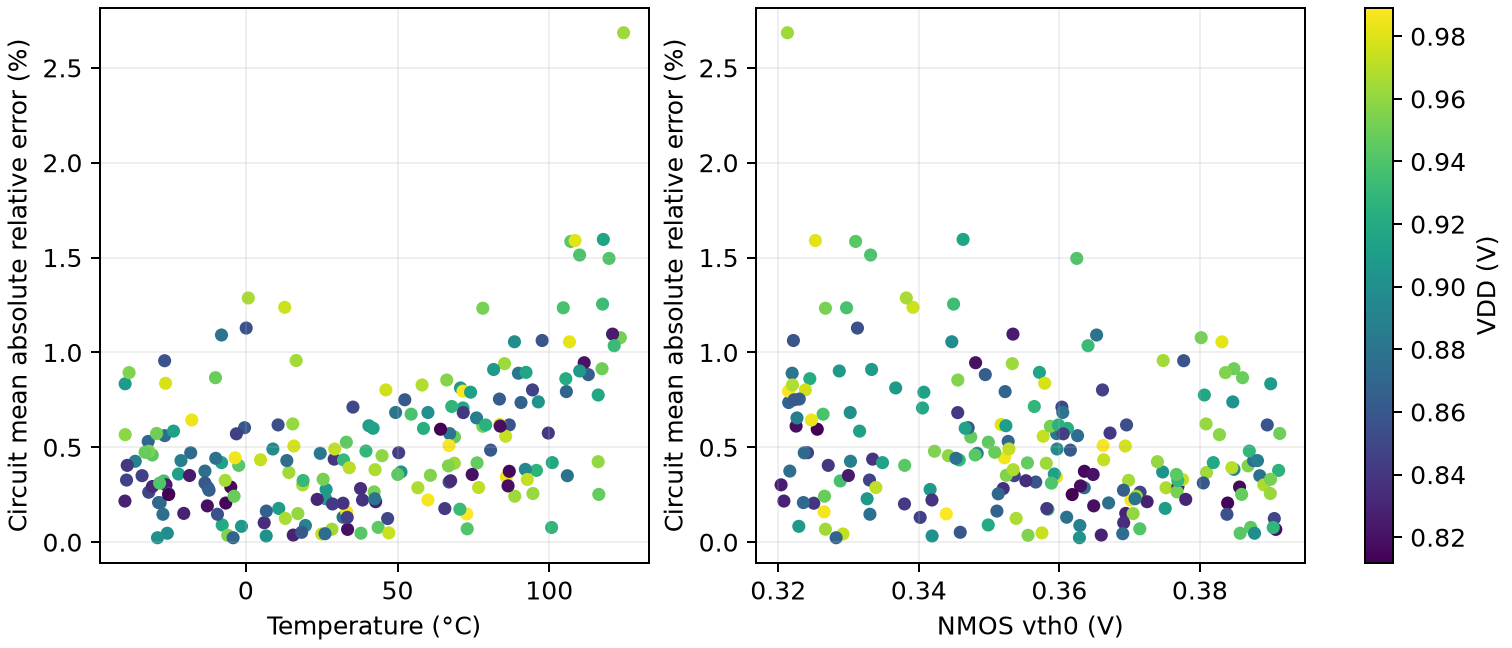
\includegraphics[width=.96\linewidth,height=.30\textheight,keepaspectratio]{figures/corner_error.png}
\caption{Each point summarizes 256 complete-circuit patterns at one corner. Color encodes VDD.}
\end{figure}

Raw predicted four-current KCL residual: median 7.57e-18 A, maximum 1.31e-12 A across gate-device queries. Before any clipping (none is applied), 0 FET predictions and 0 whole-gate predictions have negative calculated power. Source closure ensures per-device current conservation for energy calculation, but does not enforce passivity or inter-device node balance.

The principal distribution shift is between uniformly sampled individual terminal voltages and gates, whose conducting transistor terminals often lie extremely close together or to a supply rail. Small-current targets and the wide current dynamic range make raw-space R² insufficient to establish percent accuracy. Errors from individual terminals can be amplified by a low reference leakage; current signs and near-zero denominators are therefore retained rather than concealed.

Independent validation artifacts: \path|reports/circuit_reference_validation.json| and \path|code/scripts/verify_circuit_references.py| (repository-root paths). Raw execution logs are regenerated when the numerical pipeline is run. These checks use separate terminal ammeters and manually assembled gate references to compare transistor dissipated power with external-source power, plus reverse-order/fresh-input parity checks. Numerical verdict: PASSED.

\clearpage

% === 8. Limitations and improvements ===

\section{Limitations and improvements}

This is a compact-model simulation study, not measured silicon. The assigned predictive model and its ngspice implementation limit physical fidelity. Default diffusion geometry and no extracted interconnect parasitics mean layout leakage and loading are not modeled. The independent ±10\% process draws are the assignment's statistical experiment, not a calibrated foundry process distribution.

The prescribed Part B method already needs SPICE internal/output voltages at each evaluated gate corner; it is not an entirely SPICE-free node solver. Part C then replaces real inter-stage analog behavior with Boolean states. Consequently a high transistor R² does not imply 99\% gate or circuit accuracy.

Remaining improvements include better treatment of tiny body currents and signed cancellations, a gate-body residual that remains representable at zero edge voltage, and measured uncertainty on new PVT domains. The physics normalization is specific to the assigned model and is not claimed to transfer unchanged to another technology. Any targeted rail-boundary training would need to remain distinct from the brief's uniform sampling requirement. An independently validated internal-node solver would be a separate extension. Gate/circuit evaluation currents must remain excluded from fitting and model selection.

\clearpage

% === 9. Reproduction and deliverable map ===

\section{Reproduction and deliverable map}

From the submission repository root, run \texttt{bash run.sh setup}, then \texttt{bash run.sh verify}. Run \texttt{bash run.sh reproduce} to regenerate the numerical pipeline in \path|code/reproduced/|, preserving the submitted models and measurements. Shared source code and the environment lock are under \path|code/|. The submitted datasets, models, results, netlists and reports are at the repository root. Only the final 100,000-row datasets are included: Part A explicitly permits changing the initial sample count. Input-only tables and full candidate-training outputs are regenerated during reproduction rather than duplicated in this submission. Historical absolute paths in the original freeze manifests identify the original run; the verification command resolves the packaged files locally.

The ordered reproduction pipeline samples, simulates devices, trains models, checks trends, simulates gates/circuit, validates references, evaluates hierarchy, builds this report, and checks the final deliverables. Fixed seeds, CSV splits, exact dependency versions and file checksums are included. Cached successful reference simulations are keyed to their inputs and model/executable hashes.

\begingroup
\fontsize{8.5}{11}\selectfont
\setlength{\tabcolsep}{3pt}
\renewcommand{\arraystretch}{1.16}
\begin{longtable}{@{}>{\raggedright\arraybackslash}p{41.557mm} >{\raggedright\arraybackslash}p{126.334mm}@{}}
\toprule
\textbf{Deliverable} & \textbf{Location} \\
\midrule
\endfirsthead
\toprule
\textbf{Deliverable} & \textbf{Location} \\
\midrule
\endhead
\midrule\multicolumn{2}{r}{\footnotesize Continued on next page}\\
\endfoot
\bottomrule
\endlastfoot
Four 100,000-row datasets & \path|data/transistors/{case}.csv| \\
Fixed partitions and 200 corners & \path|data/splits/| and \path|data/corners.csv| \\
Example decks & \path|netlists/transistors/|, \path|netlists/gates/|, \path|netlists/circuit/parity8.cir| \\
KCL / three controlled trends & \path|reports/data_checks/| \\
16-row model comparison & \path|results/transistor_validation_models.csv| \\
Four saved models & \path|models/{case}.joblib| \\
Held-out currents and metrics & \path|results/test_predictions/| and transistor\_test*.csv \\
18-case gate table and predictions & \path|results/gate_metrics.csv| and gate\_predictions.csv \\
51,200 circuit predictions / 256-vector table & \path|results/circuit_predictions.csv| and circuit\_metrics\_by\_vector.csv \\
Shared source code / environment & \path|code/lusr/|, \path|code/scripts/|, \path|code/requirements.lock.txt| \\
Typed report / figures & \path|reports/LUSR_8bit_Parity_Leakage_Report.pdf|, \path|reports/main.tex| and accompanying figures \\
\end{longtable}
\endgroup
\vspace{2pt}

\clearpage

\section*{References}

\addcontentsline{toc}{section}{References}

Supplied Digital VLSI Design course-project brief: DVD\_ML\_PROJECT.pdf, pp. 1--4.

Supplied Project-1\_leakage\_estimation\_annotated.pdf. Slide 15 explicitly labels an illustrative equation incomplete; it is not used as a complete leakage formula.

ngspice 42 User Manual: \url{https://ngspice.sourceforge.io/docs/ngspice-42-manual.pdf}

Official ngspice control-language tutorial: \url{https://ngspice.sourceforge.io/ngspice-control-language-tutorial.html}

BSIM4 User Manual, oxide definitions: \url{https://ngspice.sourceforge.io/external-documents/models/BSIM480_Manual.pdf}

scikit-learn, common pitfalls and data leakage: \url{https://scikit-learn.org/stable/common_pitfalls.html}

scikit-learn, mean absolute percentage error: \url{https://scikit-learn.org/stable/modules/generated/sklearn.metrics.mean_absolute_percentage_error.html}

SciPy, RBFInterpolator (local neighbors and polynomial degree requirements): \url{https://docs.scipy.org/doc/scipy/reference/generated/scipy.interpolate.RBFInterpolator.html}

\end{document}
